%Shortest path problem
\section{Shortest path problem}\label{shortestPathProblem}
	For route planning, routes through a network must be optimized in regards to one or even many criteria.
	A common criteria is the \textit{travel time}. Others include cost, number of transfers or restrictions
	in transportation types.
	
	In this chapter, we will first give an informal description of the \earliestArrivalProblem. Followed by
	the \shortestPathProblem, which is equivalent to the \earliestArrivalProblem for our graph based network
	representations.
	
	Then, we introduce algorithms for solving the problem. First, for time-independent networks, then for time-dependent.
	Afterwards, we explain two solutions for combined networks, using multiple transportation modes. There, the problem
	description slightly changes by adding transportation mode restrictions.\\\\
	\begin{mydef}
		The earliest arrival problem asks for finding a \textnormal{route} in a network with following properties
		\begin{itemize}
			\item[1.] The route must start at $s$ and end at $t$.
			\item[2.] The departure time at $s$ is $\tau$.
			\item[3.] All other applicable routes must have a greater travel time, i.e. arrive later at $t$.
		\end{itemize}
		Points $s$ and $t$ are given source and target points in the network respectively. $\tau$ is the desired departure time,
		it may be ignored for a time-independent network.
	\end{mydef}
	\begin{mydef}
		Given a graph $G = (V, E)$, source and target nodes $s, t \in V$ and a desired departure time $\tau$, the shortest path
		problem asks for a path $p$ (see \defref{path}) which
		\begin{itemize}
			\item[1.] begins at $s$ and ends at $t$,
			\item[2.] has the smallest weight of all applicable paths.
		\end{itemize}
		The arrival time at $t$ is $\tau$ plus the weight of $p$. In a time-dependent
		graph $\tau$ must be used to ensure correct edge weights. The path $p$ is called \textnormal{shortest path}.
	\end{mydef}\quad\\
	Additionally, we consider a special variant of the shortest path problem:
	\begin{mydef}
		The many-to-one shortest path problem is a variation of the shortest path problem
		where the source consists of a set of source nodes $S \subseteq V$.

		The problem asks for the path $p$ that starts at the source $s \in S$ which minimizes the path weight.
	\end{mydef}

%Time-independent
\subsection{Time-independent}
	Route planning in time-independent networks is a very well studied problem.
	Many efficient solutions to the shortest path problem exists. We introduce a very basic algorithm, \dijkstra
	and a simple improvement based on heuristics, \astar.
	% Time-independent example
	\begin{figure}[!ht]
		 \begin{center}
			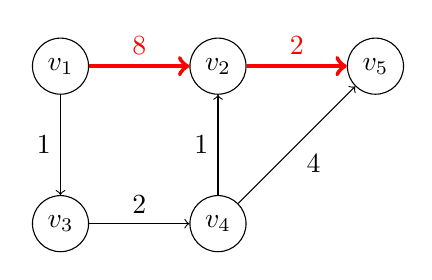
\begin{tikzpicture}[y = -1cm]
			 	% Nodes
			 	\node[circle, draw] (v1) at (0, 0) {$v_1$};
			 	\node[circle, draw] (v2) at (2, 0) {$v_2$};
			 	\node[circle, draw] (v3) at (0, 2) {$v_3$};
			 	\node[circle, draw] (v4) at (2, 2) {$v_4$};
			 	\node[circle, draw] (v5) at (4, 0) {$v_5$};
			 	
			 	% Edges
			 	\draw[ultra thick, ->, color = red] (v1) to node[above] {$8$} (v2);
			 	\draw[ultra thick, ->, color = red] (v2) to node[above] {$2$} (v5);
			 	\draw[->] (v1) to node[left] {$1$} (v3);
			 	\draw[->] (v3) to node[above] {$2$} (v4);
			 	\draw[->] (v4) to node[left] {$1$} (v2);
			 	\draw[->] (v4) to node[below right] {$4$} (v5);
			\end{tikzpicture}\qquad\qquad\qquad
			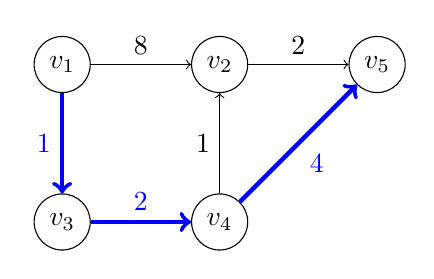
\begin{tikzpicture}[y = -1cm]
			 	% Nodes
			 	\node[circle, draw] (v1) at (0, 0) {$v_1$};
			 	\node[circle, draw] (v2) at (2, 0) {$v_2$};
			 	\node[circle, draw] (v3) at (0, 2) {$v_3$};
			 	\node[circle, draw] (v4) at (2, 2) {$v_4$};
			 	\node[circle, draw] (v5) at (4, 0) {$v_5$};
			 	
			 	% Edges
			 	\draw[->] (v1) to node[above] {$8$} (v2);
			 	\draw[->] (v2) to node[above] {$2$} (v5);
			 	\draw[ultra thick, ->, color = blue] (v1) to node[left] {$1$} (v3);
			 	\draw[ultra thick, ->, color = blue] (v3) to node[above] {$2$} (v4);
			 	\draw[->] (v4) to node[left] {$1$} (v2);
			 	\draw[ultra thick, ->, color = blue] (v4) to node[below right] {$4$} (v5);
			\end{tikzpicture}\quad\\\phantom{v}\quad\\
			\begin{tikzpicture}[y = -1cm]
			 	% Nodes
			 	\node[circle, draw] (v1) at (0, 0) {$v_1$};
			 	\node[circle, draw] (v2) at (2, 0) {$v_2$};
			 	\node[circle, draw] (v3) at (0, 2) {$v_3$};
			 	\node[circle, draw] (v4) at (2, 2) {$v_4$};
			 	\node[circle, draw] (v5) at (4, 0) {$v_5$};
			 	
			 	% Edges
			 	\draw[->] (v1) to node[above] {$8$} (v2);
			 	\draw[ultra thick, ->, color = darkgreen] (v2) to node[above] {$2$} (v5);
			 	\draw[ultra thick, ->, color = darkgreen] (v1) to node[left] {$1$} (v3);
			 	\draw[ultra thick, ->, color = darkgreen] (v3) to node[above] {$2$} (v4);
			 	\draw[ultra thick, ->, color = darkgreen] (v4) to node[left] {$1$} (v2);
			 	\draw[->] (v4) to node[below right] {$4$} (v5);
			\end{tikzpicture}
		\end{center}
		\caption{Example for a time independent network, represented by a road graph.
		The figure shows three paths from $v_1$ to $v_5$. From top left to bottom right, the path
		weights are $10$, $7$ and $6$. The last example represents the shortest path from $v_1$ to $v_5$.}
		\label{timeIndependentExample}
	\end{figure}\quad\\
	The network shown by \figref{timeIndependentExample} acts as toy example for this section.

%Dijkstra
\subsubsection{Dijkstra}
	\dijkstra \libref{dijkstra} is a simple approach to solving the shortest path problem. It can be viewed
	as the logical extension of breadth-first search (\bfs) \libref{dijkstra} in weighted graphs. The algorithm
	revolves around a priority queue where it stores neighboring nodes, sorted by their shortest path cost.
	In each round, the node with the smallest shortest path cost is \textit{relaxed}. That is, all its neighboring,
	not already relaxed, nodes are added to the queue. The algorithm terminates as soon as the target node has been relaxed.
	\algoref{dijkstra} gives a formal description.
	% Dijkstra implementation
	\IncMargin{1em}
	\begin{algorithm}
		\SetKwInOut{Input}{input}
  		\SetKwInOut{Output}{output}
  		\SetKw{Break}{break}
  		\SetKwData{undef}{undefined}\SetKwData{currentDist}{currentDist}
		\SetKwFunction{dist}{dist}\SetKwFunction{prev}{prev}
		\BlankLine
		\Input{graph $G = (V, E)$, source $s \in V$, target $t \in V$}
		\Output{shortest path from $s$ to $t$}
		\BlankLine
		\tcp{Initialization}
		\For{$v \in V$}{
			$\dist(v) \leftarrow \infty$\;
			$\prev(v) \leftarrow \undef$\;
		}
		\BlankLine
		$\dist(s) \leftarrow 0$\;
		$Q \leftarrow \{s\}$\;
		\BlankLine
		\tcp{Compute shortest paths}
		\While{$Q$ is not empty}{
			$u \leftarrow \argmin_{u' \in Q} \dist(u')$\;
			$Q \leftarrow Q \setminus \{u\}$\;
			\BlankLine
			\If{$u == t$}{
				\Break\;
			}
			\BlankLine
			\tcp{Relax $u$}
			\For{outgoing edge $(u, w, v) \in E$}{
				$\currentDist \leftarrow \dist(u) + w$\;
				\If{$\currentDist < \dist(v)$}{
					\tcp{Improve distance by using this edge}
					$\dist(v) \leftarrow \currentDist$\;
					$\prev(v) \leftarrow u$\;
					$Q \leftarrow Q \cup \{v\}$\;
				}
			}
		}
		\BlankLine
		\tcp{Extract path by backtracking}
		$p \leftarrow$ empty path\;
		$u \leftarrow t$\;
		\While{$\prev(u) \neq \undef$}{
			$w \leftarrow \dist(u) - \dist(\prev(u))$\;
			prepend $(\prev(u), w, u)$ to $p$\;
			$u \leftarrow \prev(u)$\;
		}
		prepend $s$ to $p$\;
		\Return $p$\;
		\BlankLine
		\caption{Dijkstra's algorithm for computing shortest paths in time-independent graphs.}\label{dijkstra}
	\end{algorithm}\DecMargin{1em}\quad\\\\
	To familiarize with the algorithm, we step through the execution for the graph shown by \figref{timeIndependentExample},
	with $v_1$ as source and $v_5$ as target node.
	
	The $\dist$ function, often implemented as array, stores the tentative shortest path weight to the given node.
	$\prev$ is used for path extraction at the end, it stores the parent nodes used for the shortest paths represented by $\dist$.
	The algorithm starts by initializing both collections with default values. Initially the distance to all nodes, except the source, is unknown.
	Thus, $\infty$ is used for them. $Q$ represents the list of nodes that need to be processed, usually implemented as priority queue.
	Initially, it only holds the source node $s$.
	
	In the example $Q$ is initially $\{v_1\}$. The algorithm then relaxes $v_1$ and stores distances to its neighbors:
	\begin{center}
		\begin{tabular}{CC}
			\dist(v_2) = 8	&\prev(v_2) = v_1,\\
			\dist(v_3) = 1	&\prev(v_3) = v_1
		\end{tabular}
	\end{center}
	Additionally, the queue $Q$ is updated, it is
	\begin{align*}
		Q	&= \{v_2, v_3\}.
	\end{align*}
	The next iteration of the loop starts and the node with the smallest distance is chosen, i.e. $v_3$. The node is relaxed and we receive
	\begin{center}
		\begin{tabular}{CC}
			\dist(v_4) = 3	&\prev(v_4) = v_3,\\
			\multicolumn{2}{c}{$Q = \{v_2, v_4\}.$}
		\end{tabular}
	\end{center}
	The next node is $v_4$, yielding
	\begin{center}
		\begin{tabular}{CC}
			\dist(v_2) = 4	&\prev(v_2) = v_4,\\
			\dist(v_5) = 7	&\prev(v_5) = v_4,\\
			\multicolumn{2}{c}{$Q = \{v_2, v_5\}.$}
		\end{tabular}
	\end{center}
	Note that $v_4$ improves the distance to $v_2$. The previous values for $v_2$ are overwritten and the
	tentative shortest path to $v_2$ uses $(v_4, 1, v_2)$ and not $(v_1, 8, v_2)$ anymore.
	In the next round $v_2$ is relaxed which improves the distance to $v_5$:
	\begin{center}
		\begin{tabular}{CC}
			\dist(v_5) = 6	&\prev(v_5) = v_2,\\
			\multicolumn{2}{c}{$Q = \{v_5\}.$}
		\end{tabular}
	\end{center}
	The only node left is the target node $v_5$ now. It is relaxed and the loop terminates.
	The algorithm backtracks the parent pointer
	\begin{align*}
		\prev(v_5)	&= v_2,\\
		\prev(v_2)	&= v_4,\\
		\prev(v_4)	&= v_3,\\
		\prev(v_3)	&= v_1,\\
		\prev(v_1)	&= \vundef
	\end{align*}
	and constructs the shortest path
	\begin{align*}
		p	&= (v_1, 1, v_3)(v_3, 2, v_4)(v_4, 1, v_2)(v_2, 2, v_5)
	\end{align*}
	which is the path shown by the last example in the figure.

%A*
\subsubsection{\astar and \alt}\label{alt}
	An important observation of \dijkstra is that, if it settles the shortest path distance to a node, then,
	all nodes which are closer to the source, were already settled in a previous round.
	
	Moreover, the algorithm explores the graph in all directions equally. It has no sense of \textit{goal direction}.\\\\
	The \astar algorithm \libref{alt} is a simple extension of \dijkstra which improves its efficiency by steering the
	exploration more towards the target. \figref{dijkstra_vs_astar} illustrates this by comparing the \textit{search space}
	of both algorithms. The search space of \astar is smaller and much more directed to the target node $t$.
	% A-star vs Dijkstra
	\begin{figure}[!ht]
		 \begin{center}
			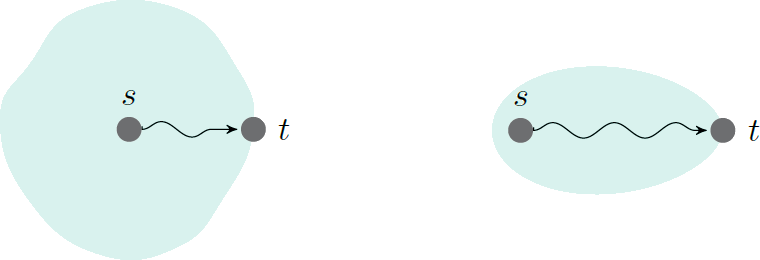
\includegraphics[scale=0.5]{res/dijkstra_vs_astar}
		\end{center}
		\caption{Schematic illustration of a query processed by \dijkstra (left) and \astar (right).
			The highlighted areas indicate the \textit{search space}, i.e. the nodes the algorithm has explored already.
			The illustration is from \libref{routePlanningOverview}.}
		\label{dijkstra_vs_astar}
	\end{figure}\quad\\
	Unfortunately, computing the exact goal direction is as hard as computing the shortest path to the target.
	Therefore, a heuristic is used to approximate the direction. The choice of the heuristic heavily depends on the underlying network.
	In the worst case, a heuristic may not improve over \dijkstra and the same search space is received. In the best case,
	the algorithm explores only the nodes on the shortest path.
	
	Such a heuristic must fulfill two properties, formulated by \defref{heuristic}.
	\begin{mydef}\label{heuristic}
		Given a graph $G = (V, E)$, a metric $\dist$ on $V$ (see \defref{metric}),
		a \textnormal{heuristic} is a function $h: V \times V \to \mathbb{R}_{\ge 0}$ which approximates $\dist$.
		The heurstic $h$ must be
		\begin{itemize}
			\item[1.] \textnormal{admissable}, i.e. never overestimate:
				\begin{align*}
					\forall u, t \in V: h(u, t) \le \dist(u, t)
				\end{align*}
			\item[2.] \textnormal{monotone}, i.e. satisfy the triangle inequality:
				\begin{align*}
					\forall t \in V\,\forall (u, w, v) \in E: h(u, t) \le w + h(v, t)
				\end{align*}
		\end{itemize}
	\end{mydef}\quad\\
	Given such a heuristic $h$, the \astar algorithm is received by adjusting \textbf{line 7} of \algoref{dijkstra} to
	\begin{align*}
		u \leftarrow \argmin_{u' \in Q} \dist(u') + h(u', t).
	\end{align*}
	This will prefer nodes that are estimated to be closer to the target before others. By that, the algorithms search space
	first expands into a direction that minimizes the distance according to the heuristic $h$.\\\\
	A common choice for a simple heuristic is the \textit{as-the-crow-flies} metric (see \defref{asTheCrowFlies}).
	The properties are easily verified. A theoretically shortest path has the shortest possible distance and uses
	the fastest available transportation mode. This is exactly the path represented by the \textit{straight-line} distance,
	computed by the \textit{as-the-crow-flies} metric. It can thus never overestimate. It is also trivially monotone since it is a metric,
	i.e. the triangle inequality holds for all elements.
	
	A heuristic is a good choice if it approximates the actual shortest path distance well. As such, the \textit{as-the-crow-flies} heuristic works well
	on networks with a high connectivity in all directions. For example a residential area of a city without one way streets. Unfortunately, in road
	networks, the common case is to first drive into the opposite direction in order to reach a fast highway. This even gets worse on networks
	where the importance of nodes heavily differ, such as public transit networks. For train networks, the typical case is that one first needs
	to travel to a main station. This is obviously due to a main station having a much better connectivity and faster trains available.
	Because of that, the effectiveness of \textit{as-the-crow-flies} is very limited on such networks.\\\\
	The \textit{landmark heurstic} partially solves the issue. An \astar algorithm using the landmark heuristic is called \alt \libref{alt},
	which stands for \textit{landmarks and triangle inequality}.
	
	The heuristic provides a more generic approach by approximating the distance
	between nodes $u$ and $v$ by using precomputed distances with pre-determined nodes $l$, called \textit{landmarks}.
	\begin{mydef}\label{alt_heuristic}
		Given a set of landmarks $L \subseteq V$, the heuristic $\landmarks$ is defined by
		\begin{align*}
			\landmarks(u, v)	&= \max_{l \in L} \left(\max \{\dist(u, l) - \dist(v, l), \dist(l, v) - \dist(l, u)\}\right).
		\end{align*}
	\end{mydef}\quad\\
	Obviously, the heuristic improves if the set of landmarks is increased. However, actual shortest path distances from all landmarks
	to all other nodes in the graph must be precomputed. With an increasing amount of landmarks the precomputation might not
	be feasible anymore because it takes too long or consumes too much space. Note that if $L = V$, the heuristic becomes the
	actual shortest path distance function, i.e. $\landmarks = \dist$.
	
	In practice, an amount between $20$ and $50$ randomly chosen nodes seems to be a good compromise.
	Refer to \libref{alt} for a detailed analysis.\\\\
	The computation of the actual shortest path distances, to and from the landmarks, can be done by using \dijkstra. But, instead of
	running the algorithm for all pairs of nodes, the distances can be obtained with two runs only. Therefore, the algorithm is slightly modified by dropping
	\textbf{lines 9} and \textbf{10}, such that the algorithm relaxes the whole network. By that, a single run of \dijkstra with a landmark $l$ as source,
	computes the distances $\dist(l, v)$ to all nodes $v$ in the network. By reversing the graph, i.e. edges $(u, w, v)$ become $(v, w, u)$, the distances to
	the landmarks can be obtained analogously with $l$ as source again. Depending on the graph implementation, reversal can be done
	in $\mathcal{O}(1)$ by only implicitly reversing the edges.

%Time-dependent
\subsection{Time-dependent}\label{time_dependent_sec}
	Approaches designed for time-independent networks, such as \alt, have an important drawback. Optimization is always done on
	assuming that edge costs are constant. However, in a time-dependent network, this is not the case. The weight of an edge is
	dependent on the departure time, which is not known in advance.\\\\
	\dijkstra and its variants \astar and \alt can easily be adapted to also work in time-dependent networks by taking the departure
	time into consideration when computing the weight of an edge. However, their effectiveness is very limited.
	Nonetheless, they where used for a long time for time-dependent networks too. With increasing research on route
	planning in time-dependent networks, more effective algorithms, such as \transferPatterns \libref{transferPatterns}
	and \csa \libref{csa}, were developed. Many of them do not use graphs and prefer data-structures that are designed
	for time-dependent data, such as \textit{timetables} (see \sectionref{timetable_sec}).

%Connection scan
\subsubsection{Connection scan}\label{csa}
	Connection scan (\csa) \libref{csa} is an algorithm for route planning specially designed for time-dependent networks,
	such as public transit networks. It processes the network represented as timetable, as defined by \defref{timetable}.\\\\
	The algorithm is very simple. All connections of the timetable are sorted by their departure time.
	Give a query connections are explored increasing in their departure time. The algorithm is fast primarily due to the fact that
	connections can be maintained in a simple array. In contrast to \dijkstra, it does not need to maintain a priority queue or
	other more complex data-structures. Arrays are heavily optimized and benefit from a lot of effects, like cache locality \libref{cacheLocality}.
	% CSA implementation
	\IncMargin{1em}
	\begin{algorithm}
		\SetKwInOut{Input}{input}
  		\SetKwInOut{Output}{output}
  		\SetKw{Break}{break}
  		\SetKwData{undef}{undefined}
		\BlankLine
		\Input{timetable $(S, T, C, F)$, source $s \in S$, target $t \in S$, departure time $\tau$}
		\Output{shortest path from $s$ to $t$}
		\BlankLine
		\tcp{Initialization}
		\lFor{$u \in S$}{
			$S[u] \leftarrow \infty$
		}
		\lFor{$o \in T$}{
			$T[o] \leftarrow \undef$
		}
		\lFor{$u \in S$}{
			$J[u] \leftarrow (\undef, \undef, \undef)$
		}
		\BlankLine
		\For{$f = (u_{\dep}, d, u_{\arr}) \in F : u_{\dep} = s$}{
			$S[u_{\arr}] \leftarrow \tau + d$\;
			$J[u_{\arr}] \leftarrow (\undef, \undef, f)$\;
		}
		\BlankLine
		\tcp{Explore connections increasing in departure time}
		$c_0 \leftarrow \argmin_{(u_{\dep}, u_{\arr}, \tau_{\dep}, \tau_{\arr}, o) \in C : \tau_{\dep} \ge \tau} \tau_{\dep}$\;
		\For{$c = (u_{\dep}, u_{\arr}, \tau_{\dep}, \tau_{\arr}, o) \in C$ increasing by $\tau_{\dep}$, starting from $c_0$}{
			\If{$\tau_{\dep} \ge S[t]$}{
				\Break\;
			}
			\BlankLine
			\If{$T[o] \neq \undef \lor \tau_{\dep} \ge S[u_{\dep}]$}{
				\If{$T[o] == \undef$}{
					$T[o] \leftarrow c$\;
				}
				\If{$\tau_{\arr} < S[u_{\arr}]$}{
					\For{$f = (v_{\dep}, d, v_{\arr}) \in F : v_{\dep} = u_{\arr}$}{
						\If{$\tau_{\arr} + d < S[v_{\arr}]$}{
							$S[v_{\arr}] \leftarrow \tau_{\arr} + d$\;
							$J[v_{\arr}] \leftarrow (T[o], c, f)$\;
						}
					}
				}
			}
		}
		\BlankLine
		\tcp{Extract path by backtracking}
		$p \leftarrow$ empty path\;
		$u \leftarrow t$\;
		\While{$c_{\enter} \neq \undef : (c_{\enter}, c_{\exit}, f) = J[u]$}{
			prepend $f$ to $p$\;
			prepend the part of the trip between $c_{\enter}$ and $c_{\exit}$ to $p$\;
			$u \leftarrow v_{\dep} : (v_{\dep}, v_{\arr}, \tau'_{\dep}, \tau'_{\arr}, o) = c_{\enter}$\;
		}
		prepend $f : (\undef, \undef, f) = J[s]$ to $p$\;
		\Return $p$\;
		\BlankLine
		\caption{Connection scan algorithm for computing shortest paths in time-dependent networks, represented by timetables.}\label{csa_algo}
	\end{algorithm}\DecMargin{1em}\quad\\\\
	\algoref{csa_algo} shows the full connection scan algorithm. The array $S$ stores for each stop the currently best arrival time.
	$T$ associates for each trip the first connection it is taken with. $J$ is used for path extraction and memorizes for each stop a
	segment of a trip, consisting of enter and exit connections $c_{\enter}$ and $c_{\exit}$ respectively, and a footpath $f$:
	\begin{align*}
		(c_{\enter}, c_{\exit}, f)
	\end{align*}
	It represents a path which takes the segment of the trip starting at $c_{\enter}$, ending at $c_{\exit}$ and then taking the footpath $f$ from
	the arrival stop of $c_{\exit}$. Such an entry is associated to the arrival stop of the footpath $f$, always representing the parent path
	that results in the current best arrival time for the corresponding stop.\\\\
	The algorithm starts by initializing the arrays with default values and relaxing all initial footpaths. Connections are then explored
	increasing in their departure time, starting from the first connection $c_0$ that starts after the departure time $\tau$. \textbf{Line 7}
	is typically implemented as \textit{binary search} \libref{binarySearch} on a sorted array of connections $C$.
	
	\textbf{Line 9} is the stopping criteria, which lets the algorithm terminate once a connection departs after the current best arrival
	time at the target $t$. Since connections are explored increasing in time, it is impossible that a connection can improve on the
	arrival time anymore.
	
	\textbf{Line 11} will only explore a connection if a previous connection of the same trip was already used, indicating
	traveling without a transfer; or if it was already possible to arrive at the stop earlier with a previous connection, indicating
	a transfer at this stop.
	
	A connection is then only relaxed if it improves the arrival time at its arrival stop, represented by \textbf{line 14}.
	If so, all outgoing footpaths are explored. A footpath represents exiting the vehicle, walking to the arrival stop of the footpath
	ready for entering another vehicle. Note that self-loop footpaths must be contained in timetables (compare to \defref{timetable}),
	making it possible to transfer at one stop.
	
	\textbf{Line 16} only considers footpaths that improve the arrival time at the corresponding stop. \textbf{Line 18} stores the path
	represented by taking this connection and the footpath.\\\\
	For an example, we refer to the schedule of \figref{simpleTransitGraphExample} again. The corresponding timetable is
	explained in \sectionref{timetable_sec}, we use the same notion again.
	It consists of five connections, denoted by $c_1, c_2, c_3, c_4$ and $c_5$,
	sorted by departure time. We assume only the three self-loop footpaths on the stops $f$, $o$ and $k$.
	
	Assume a query from \freiburg, represented by stop $f$ to \karlsruhe, represented by $k$, with a departure time of
	$\tau = \timef{3}{50}{pm}$. The initial configuration after \textbf{line 3} is
	\begin{align*}
		S[f]		&= S[o] = S[k] = \infty,\\
		T[t_{104}]	&= T[t_{17024}] = T[t_{17322}] = T[t_{79}] = \vundef,\\
		J[f]		&= J[o] = J[k] = (\vundef, \vundef, \vundef).
	\end{align*}
	Then the footpath $(f, 300, f)$ departing at \freiburg is relaxed, resulting in
	\begin{align*}
		S[f]	&= \timef{3}{55}{pm},\\
		J[f]	&= (\vundef, \vundef, (f, 300, f)).
	\end{align*}
	Connections are now explored increasing in departure time, starting with
	\begin{align*}
		c_1	&= (f, o, \timef{3}{56}{pm}, \timef{4}{28}{pm}, t_{104}).
	\end{align*}
	The connection is considered since we already arrived at \freiburg before \timef{3}{56}{pm}. The trip is set and the
	footpath at \offenburg is relaxed, yielding
	\begin{align*}
		T[t_{104}]	&= c_1,\\
		S[o]		&= \timef{4}{33}{pm},\\
		J[o]		&= (c_1, c_1, (o, 300, o)).
	\end{align*}
	The next connection is
	\begin{align*}
		c_2	&= (f, o, \timef{4}{03}{pm}, \timef{4}{50}{pm}, t_{17024}).
	\end{align*}
	However, it induces no changes, as the previous connection already arrived at \offenburg earlier.
	The algorithm continues by exploring
	\begin{align*}
		c_3	&= (o, k, \timef{4}{29}{pm}, \timef{4}{58}{pm}, t_{104}).
	\end{align*}
	The connection is considered because the trip $t_{104}$ was used before already, indicating that the trip can be taken without transferring.
	Else it would not be applicable, since the current best arrival time at \offenburg, including the transfer duration of $5$ minutes,
	is \timef{4}{33}{pm}, which is after the departure time of $c_3$. The changes are
	\begin{align*}
		S[k]		&= \timef{5}{03}{pm},\\
		J[k]		&= (c_1, c_3, (k, 300, k)).
	\end{align*}
	In the next iteration
	\begin{align*}
		c_4	&= (o, k, \timef{4}{35}{pm}, \timef{5}{19}{pm}, t_{17322})
	\end{align*}
	is considered, again inducing no changes. The algorithm then terminates exploration since the last connection
	\begin{align*}
		c_5	&= (k, f, \timef{7}{10}{pm}, \timef{8}{10}{pm}, t_{79})
	\end{align*}
	departs after the current best arrival time at \karlsruhe, which is $S[k] = \timef{5}{03}{pm}$.
	
	Path construction is straightforward, it is
	\begin{align*}
		J[k]	&= (c_1, c_3, (k, 300, k)),\\
		J[f]	&= (\vundef, \vundef, (f, 300, f)),
	\end{align*}
	which yields the path which takes
	\begin{itemize}
		\item[] the footpath from \freiburg to \freiburg,
		\item[] $t_{104}$ starting with $c_1$ to $c_3$, which is using the \ticef from \freiburg to \karlsruhe,
		\item[] and a final footpath from \karlsruhe to \karlsruhe.
	\end{itemize}
	The earliest arrival time at \karlsruhe is $S[k] = \timef{5}{03}{pm}$.
	
%Multi-modal
\subsection{Multi-modal}
	So far, all presented route planning algorithms are limited to networks only consisting routes of one transportation mode,
	for example a train network. We only distinguished between time-independent and time-dependent networks. However, in practice
	we want to plan routes involving multiple transportation modes. For example using a bicycle to drive to the next train main station,
	using the road network, and then entering a train.\\\\
	To represent transportation mode possibilities in the networks, we slightly modify our models. All edges in graph based models
	get transportation mode labels, formalized by \defref{multiModalGraph}.
	\begin{mydef}\label{multiModalGraph}
		Given a set of transportation mode labels $M$, a \textnormal{\multiModal graph} $G = (V, E)$ is
		a graph with a label function
		\begin{align*}
			\mode: E \to \{S \subseteq M\}
		\end{align*}
		that assigns to each vertex a set of available transportation modes.
	\end{mydef}\quad\\
	In our implementation in \cobweb we use the modes
	\begin{align*}
		M	&= \{\car, \bike, \foot, \tram\}.
	\end{align*}
	The \textit{timetable} model is adjusted by assigning all connections the mode $\tram$ and
	all footpaths \foot.\\\\
	Another difficulty of \multiModal routing is that, in practice, it is usually not be applicable to change transportation modes arbitrarily.
	User have different requirements and preferences regarding the change of modes. For example, it might not be possible to
	use a car right after traveling with a tram and then leaving it at a train station before continuing the journey using a train.
	If the model does not account for this, the algorithm should not be allowed to pick such a route.\\
	% Transportation mode automata example
	\begin{figure}[!ht]
		\begin{center}
			\begin{tikzpicture}[y = -1cm]
			 	% Nodes
			 	\node[initial, accepting, state] (q0) at (0, 0) {\phantom{v}};
			 	\node[accepting, state] (q1) at (2, 0) {\phantom{v}};
			 	\node[accepting, state] (q2) at (4, 0) {\phantom{v}};
			 	
			 	% Edges
			 	\draw[thick, ->] (-1, 0) to (q0);
			 	\draw[thick, ->] (q0) to [loop above] node[above] {\foot} (q0);
			 	\draw[thick, ->] (q0) to node[above] {$\foot$} (q1);
			 	\draw[thick, ->] (q0) to [bend right] node[below] {$\foot$} (q2);
			 	\draw[thick, ->] (q1) to [loop above] node[above] {\tram} (q1);
			 	\draw[thick, ->] (q1) to node[above] {$\tram$} (q2);
			 	\draw[thick, ->] (q2) to [loop above] node[above] {\car} (q2);
			\end{tikzpicture}
		\end{center}
		\caption{Automaton representing transportation mode constraints.}
		\label{transportationModeAutomataExample}
	\end{figure}\quad\\
	Applicable transportation mode sequences are typically represented as languages of
	automata (see \sectionref{automaton_sec}) \libref{labelShortestPath}. \figref{transportationModeAutomataExample} shows an example.
	The automaton accepts words consisting of routes that
	\begin{itemize}
		\item[1.] are empty,
		\item[2.] only use \foot,
		\item[3.] use the \tram after walking to a stop,
		\item[4.] use the \car after walking to a stop and using the \tram, and
		\item[5.] use the \car directly after walking.
	\end{itemize}
	A route that takes the \tram after using a \car is not accepted by the automaton and thus, not applicable.\\\\
	The search of shortest paths, restricted to such transportation mode automata, is called
	the \labelConstrainedShortestPathProblem \libref{labelShortestPath} (\lcspp). Common algorithms, like \dijkstra, \astar and \alt, were
	adapted and analyzed with respect to the \lcspp \libref{labelShortestPath, alt, lcsppShortcuts}.\\\\
	However, we will study two algorithms that are restricted to fixed languages, not accepting arbitrary automata.
	First, we show a simple extension of \dijkstra and its variants that adapts the algorithm for \multiModal route planning.
	Afterwards, we present a generic approach to combine any \uniModal algorithms for limited \multiModal route planning.

%Modified Dijkstra
\subsubsection{Modified Dijkstra}\label{modifiedDijkstra}
	In order to adapt \dijkstra and its variants \astar and \alt for \multiModal graphs (see \defref{multiModalGraph}), the algorithm
	needs to account for the labels at edges.\\\\
	Given a \multiModal graph, a source $s$ and a target $t$, and a set of available transportation modes
	\begin{align*}
		S	\subseteq \{\car, \bike, \foot, \tram\} = M
	\end{align*}
	The modified \dijkstra computes a shortest path $p$ from $s$ to $t$ which does only use
	edges labeled with available modes, i.e.
	\begin{align*}
		\forall e \in p: \mode(e) \subseteq S.
	\end{align*}
	Therefore, we adjust \textbf{line 11} of \algoref{dijkstra} to only consider outgoing edges such that
	\begin{align*}
		e = (u, w, v) \in E : \mode(e) \subseteq S.
	\end{align*}
	When multiple transportation modes are available, such as $\{\bike, \car\}$, the edge weight is not static anymore,
	as a \car can travel the distance faster than a \bike. To break the ties, we always choose the fastest transportation mode,
	referring to the order
	\begin{align*}
		\foot \sqsubset \bike \sqsubset \tram \sqsubset \car.
	\end{align*}
	The edge weight $w$ in \textbf{line 11} is then computed as if the fastest, on this edge available, transportation mode is used:
	\begin{align*}
		\max\nolimits_{\sqsubset} \mode(e)
	\end{align*}\quad\\
	% Modified Dijkstra transportation mode automaton
	\begin{figure}[!ht]
		\begin{center}
			\begin{tikzpicture}[y = -1cm]
			 	% Nodes
			 	\node[initial, accepting, state] (q0) at (0, 0) {\phantom{v}};
			 	\node[state] (q1) at (4, 0) {\phantom{v}};
			 	
			 	% Edges
			 	\draw[thick, ->] (-1, 0) to (q0);
			 	\draw[thick, ->] (q0) to [loop above] node[above] {$m \in S$} (q0);
			 	\draw[thick, ->] (q0) to node[above] {$m' \in M \setminus S$} (q1);
			 	\draw[thick, ->] (q1) to [loop above] node[above] {$m' \in M \setminus S$} (q1);
			\end{tikzpicture}
		\end{center}
		\caption{The transportation mode constraints of \dijkstra, adapted to \multiModal routing.}
		\label{modifiedDijkstraModesAutomaton}
	\end{figure}
	The modified \dijkstra accepts the transportation mode model shown by \figref{modifiedDijkstraModesAutomaton}.\\\\
	While this modification works perfectly fine for \dijkstra, it does impair the effectiveness of \astar and \alt. The problem is that
	the heuristic of \astar can not know the transportation mode restrictions $S$ beforehand. Because of that, a heuristic must
	always assume that the fastest possible transportation mode is chosen. Else, it might be possible that the actual shortest
	path uses a faster mode than the heuristic assumed, in which case the
	heuristic would overestimate the travel time and violate \defref{heuristic}.
	
	For $\asTheCrowFlies$ this means that it must assume that the straight-line distance is traveled using a \car, or more general:
	\begin{align*}
		\max\nolimits_{\sqsubset} M
	\end{align*}
	For \alt all precomputation must be done under the assumption that, at query time, there are no transportation
	mode restrictions, i.e.
	\begin{align*}
		S	&= M.
	\end{align*}
	The actual impact on the effectiveness heavily depends on the type of network. It has no effect at all, if all edges on
	the shortest path for $S = M$ can also be taken with the actual restricted version of $S$. It gets worse if edges are
	not available anymore, for example a highway that can not be taken for $S = \{\foot\}$, although the heuristic assumed
	it can be taken using a \car.
	
	In a typical road network most edges support all road-type transportation modes, i.e. $\{\foot, \bike, \car\}$. The most
	common exceptions are highways, pedestrian zones and bikeways. However, the latter two do typically not cover big distances
	and a regular road connecting the same locations is often available too. Because of that \astar and \alt typically perform worse
	only on long-distance routes, which make heavy usage of highways, if the transportation modes are restricted to modes
	not available on highways. A similar observation can be done for combined networks, like a link graph (see \sectionref{linkGraph_sec}).\\\\
	For \alt this problem can be tackled by precomputing the distances to the landmarks for every possible transportation mode
	restriction $S$ individually. However, this results in
	\begin{align*}
		|\mathcal{P}(M)|	&= 2^{|M|}
	\end{align*}
	combinations, which is usually not feasible.

%Access nodes
\subsubsection{Access nodes}\label{accessNodes}
	Often, combining multiple networks of different types into one representation, such as a graph, is not appropriate.
	We have seen that graph representations for public transit networks dramatically scale in size, due to
	representing time information. A timetable is more suited for such a network type and algorithms optimized to a
	specific network type, such as \csa, perform much better than a generic approach like \dijkstra.\\\\
	In this section, we elaborate on a generic technique that allows to combine any networks with corresponding algorithms
	for a restricted variant of the \shortestPathProblem. We describe the algorithm by combining a road with a public transit
	network, using the \multiModal variant of \alt and \csa respectively. The general technique is known as \accessNodeRouting (\anr)
	\libref{accessNodeRouting, routePlanningOverview}.\\\\
	Given a source and a destination node in the road network, we first compute \textit{access nodes}.
	Those are nodes where we will switch from the road into the public transit network. Therefore, the access nodes
	are computed as the k-nearest neighbors (see \defref{kNearestNeighborsDef}) for both, the source and the destination node,
	in the public transit network. The amount $k$ should be kept small in order to keep query time low, we use $3$ in our implementation.
	
	In the best case, the access nodes are \textit{important}, i.e. they maximize the amount of shortest paths, from the
	source to the destination, of which they are part of. Because of that, typically they are precomputed, using a ranking among the
	nodes. For example, a train main station is preferred over a small tram stop. The computation can be optimized further by using
	heuristics and techniques like \alt were some paths are already precomputed. See \libref{accessNodeRouting} for details on
	how to obtain \textit{good} access nodes.
	
	Given the access nodes for source and destination, a path is computed piecewise, by computing shortest paths from
	\begin{itemize}
		\item[1.] the source to all its access nodes,
		\item[2.] the access nodes of the source to all access nodes of the destination, and
		\item[3.] the access nodes of the destination to the destination.
	\end{itemize}
	We denote the corresponding sets of paths by $P_s$, $P_{st}$ and $P_t$ respectively. The resulting path is chosen
	as the concatenation of paths from those sets, such that the cost is minimized. That is, we receive a path
	\begin{align*}
		p	&= p_1p_2p_3
	\end{align*}
	with $p_1 \in P_s, p_2 \in P_{st}$ and $p_3 \in P_t$ such that
	\begin{align*}
		\dest(p_1)	&= \src(p_2),\\
		\dest(p_2)	&= \src(p_3).
	\end{align*}
	Of all paths satisfying this constraints, $p$ is chosen as the path with the smallest cost. Additionally, we consider the shortest path $q$
	between the source and destination that only uses the road network. The final path is again the one with the smaller cost.
	\figref{accessNodesScheme} illustrates the scheme of this approach.
	% Access Nodes Scheme
	\begin{figure}[!ht]
		 \begin{center}
			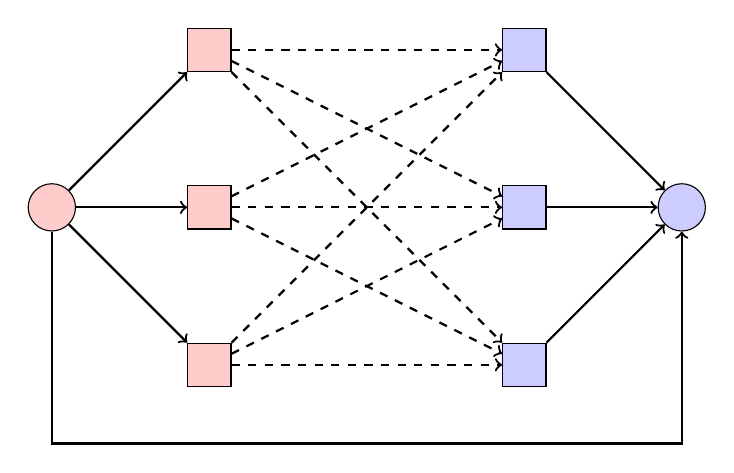
\begin{tikzpicture}[y = -1cm]
			 	% Source
			 	\node[minimum size=6mm, circle, draw, fill=red!20] (s) at (0, 2) {};
			 	
			 	% Source access nodes
			 	\node[minimum size=5.5mm, rectangle, draw, fill=red!20] (sa1) at (2, 0) {};
			 	\node[minimum size=5.5mm, rectangle, draw, fill=red!20] (sa2) at (2, 2) {};
			 	\node[minimum size=5.5mm, rectangle, draw, fill=red!20] (sa3) at (2, 4) {};
			 	
			 	% Destination access nodes
			 	\node[minimum size=5.5mm, rectangle, draw, fill=blue!20] (ta1) at (6, 0) {};
			 	\node[minimum size=5.5mm, rectangle, draw, fill=blue!20] (ta2) at (6, 2) {};
			 	\node[minimum size=5.5mm, rectangle, draw, fill=blue!20] (ta3) at (6, 4) {};
			 	
			 	% Destination
			 	\node[minimum size=6mm, circle, draw, fill=blue!20] (t) at (8, 2) {};
			 	
				% Edges
			 	% Source to access nodes
			 	\draw[thick, ->] (s) to (sa1);
			 	\draw[thick, ->] (s) to (sa2);
			 	\draw[thick, ->] (s) to (sa3);
			 	
			 	% Access to access nodes
			 	\draw[thick, dashed, ->] (sa1) to (ta1);
			 	\draw[thick, dashed, ->] (sa1) to (ta2);
			 	\draw[thick, dashed, ->] (sa1) to (ta3);
			 	
			 	\draw[thick, dashed, ->] (sa2) to (ta1);
			 	\draw[thick, dashed, ->] (sa2) to (ta2);
			 	\draw[thick, dashed, ->] (sa2) to (ta3);
			 	
			 	\draw[thick, dashed, ->] (sa3) to (ta1);
			 	\draw[thick, dashed, ->] (sa3) to (ta2);
			 	\draw[thick, dashed, ->] (sa3) to (ta3);
			 	
			 	% Access nodes to destination
			 	\draw[thick, ->] (ta1) to (t);
			 	\draw[thick, ->] (ta2) to (t);
			 	\draw[thick, ->] (ta3) to (t);
			 	
			 	% Source to destination
			 	\draw [thick, ->] (s) |- ++(8, 3) -- (t);
			\end{tikzpicture}
		\end{center}
		\caption{Scheme of \accessNodeRouting. Circular nodes represent the source and destination node,
		rectangular nodes are their corresponding access nodes. Solid edges indicate shortest paths in the first network,
		dashed lines are in the second network.}
		\label{accessNodesScheme}
	\end{figure}\quad\\
	The accepted transportation mode model is shown by \figref{accessNodesModesAutomaton}.
	% Access Nodes transportation mode automaton
	\begin{figure}[!ht]
		\begin{center}
			\begin{tikzpicture}[y = -1cm]
			 	% Nodes
			 	\node[initial, accepting, state] (q0) at (0, 0) {\phantom{v}};
			 	\node[state] (q1) at (3.5, 0) {\phantom{v}};
			 	\node[state] (q2) at (7, 0) {\phantom{v}};
			 	\node[accepting, state] (q3) at (10.5, 0) {\phantom{v}};
			 	
			 	% Edges
			 	\draw[thick, ->] (-1, 0) to (q0);
			 	\draw[thick, ->] (q0) to node[above] {$w_1 \in \mathcal{L}(A)$} (q1);
			 	\draw[thick, ->] (q1) to node[above] {$w_2 \in \mathcal{L}(B)$} (q2);
			 	\draw[thick, ->] (q2) to node[above] {$w_3 \in \mathcal{L}(A)$} (q3);
			 	\draw[thick, ->] (q0) to [bend right] node[below] {$w_4 \in \mathcal{L}(A)$} (q3);
			\end{tikzpicture}
		\end{center}
		\caption{The transportation mode constraints of \accessNodeRouting with two networks. $A$ represents the transportation
		mode model accepted by the algorithm on the first network, $B$ refers to the automaton of the algorithm on the second network.}
		\label{accessNodesModesAutomaton}
	\end{figure}\quad\\
	Note that the resulting path is not necessarily a valid solution to the \shortestPathProblem anymore. A correct solution may not even contain any
	of the used access nodes. However, if access nodes are chosen well, the resulting path is likely to be appropriate and a good approximation
	to the actual solution.